\normaltrue \difficilefalse \tdifficilefalse
\correctiontrue

%\UPSTIidClasse{11} % 11 sup, 12 spé
%\newcommand{\UPSTIidClasse}{12}

\exer{Train simple $\star$ \label{CIN:03:C2:06:28}}
\setcounter{question}{0}\marginnote{\xpComp{CIN}{03}}%\UPSTIcompetence[2]{A3-05}
%\UPSTIcompetence[2]{C2-06}
\index{Compétence C2-06}\index{Compétence CIN-03}
\index{Train d'engrenages simple}
\ifcorrection
\else
\marginnote{\textbf{Pas de corrigé pour cet exercice.}}
\fi

\ifprof
\else
Soit le train épicycloïdal suivant. 
\begin{marginfigure}
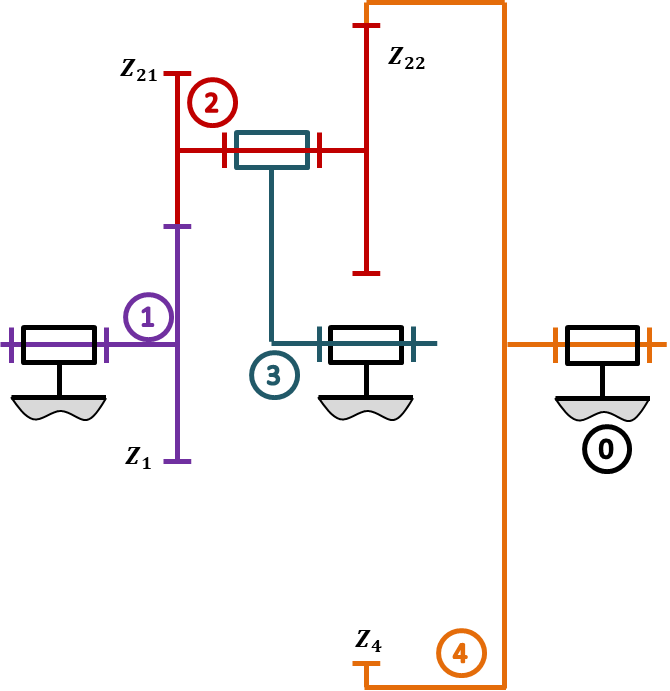
\includegraphics[width=.7\linewidth]{28_01}
\end{marginfigure}
\fi


\question{Tracer le graphe des liaisons.}
\ifprof
\else
\fi

\question{Déterminer $\omega_{40}$ en fonction de  $\omega_{30}$ et $\omega_{10}$.}
\ifprof ~\\

 En bloquant le porte satellite, on a : $\dfrac{\omega_{43}}{\omega_{13}}=-\dfrac{Z_{1}Z_{22}}{Z_{21}Z_{4}}$.
  On a donc, 
  $\dfrac{\omega_{40}+\omega_{03}}{\omega_{10}+\omega_{03}}=-\dfrac{Z_{1}Z_{22}}{Z_{21}Z_{4}}$
  $\Leftrightarrow \omega_{40}+\omega_{03}=-\dfrac{Z_{1}Z_{22}}{Z_{21}Z_{4}}\left( \omega_{10}+\omega_{03} \right)$
  $\Leftrightarrow \omega_{40}=-\dfrac{Z_{1}Z_{22}}{Z_{21}Z_{4}}\left( \omega_{10}+\omega_{03} \right)-\omega_{03}$
    $\Leftrightarrow \omega_{40}=-\dfrac{Z_{1}Z_{22}}{Z_{21}Z_{4}}\left( \omega_{10}+\omega_{03} \right)+\omega_{30}$
      $\Leftrightarrow \omega_{40}=-\dfrac{Z_{1}Z_{22}}{Z_{21}Z_{4}}\omega_{10}+\omega_{30}\left( 1+\dfrac{Z_{1}Z_{22}}{Z_{21}Z_{4}} \right)$.
\else
\fi

\question{On suppose que $\omega_{40}$ est bloqué. Exprimer le rapport $\dfrac{\omega_{30}}{\omega_{10}}$.}
\ifprof~\\
$0=-\dfrac{Z_{1}Z_{22}}{Z_{21}Z_{4}}\omega_{10}+\omega_{30}\left( 1+\dfrac{Z_{1}Z_{22}}{Z_{21}Z_{4}} \right)$

$\Leftrightarrow \dfrac{Z_{1}Z_{22}}{Z_{21}Z_{4}}\omega_{10}=\omega_{30}\left( 1+\dfrac{Z_{1}Z_{22}}{Z_{21}Z_{4}} \right)$


$\Leftrightarrow \dfrac{\omega_{30}}{\omega_{10}} 
= \dfrac{\dfrac{Z_{1}Z_{22}}{Z_{21}Z_{4}}}{ 1+\dfrac{Z_{1}Z_{22}}{Z_{21}Z_{4}} }
= \dfrac{Z_{1}Z_{22}}{ Z_{21}Z_{4}+Z_{1}Z_{22} }$.
\else
\fi

\ifprof
\else

\marginnote{Corrigé voir \ref{CIN:03:C2:06:28}.}

\fi